\documentclass[12pt,a4paper]{article}



% --- Paquetes de Idioma y Formato ---

\usepackage[utf8]{inputenc}

\usepackage[spanish, es-tabla]{babel}

\usepackage[margin=2.5cm]{geometry}

\usepackage{setspace}

\onehalfspacing

\usepackage{parskip}

\usepackage[hidelinks]{hyperref}



% --- Paquetes de Imágenes ---

\usepackage{graphicx}

\graphicspath{ {./imagenes/} } % Busca en tu carpeta 'imagenes'



% --- Configuración de la Portada ---

\title{

    \vspace{2cm} % Espacio superior

    {\Huge \textbf{Informe Previo TFG: Agentes Autónomos y Sistemas Multi-Agente (MAS)}} \\[1.5cm]

    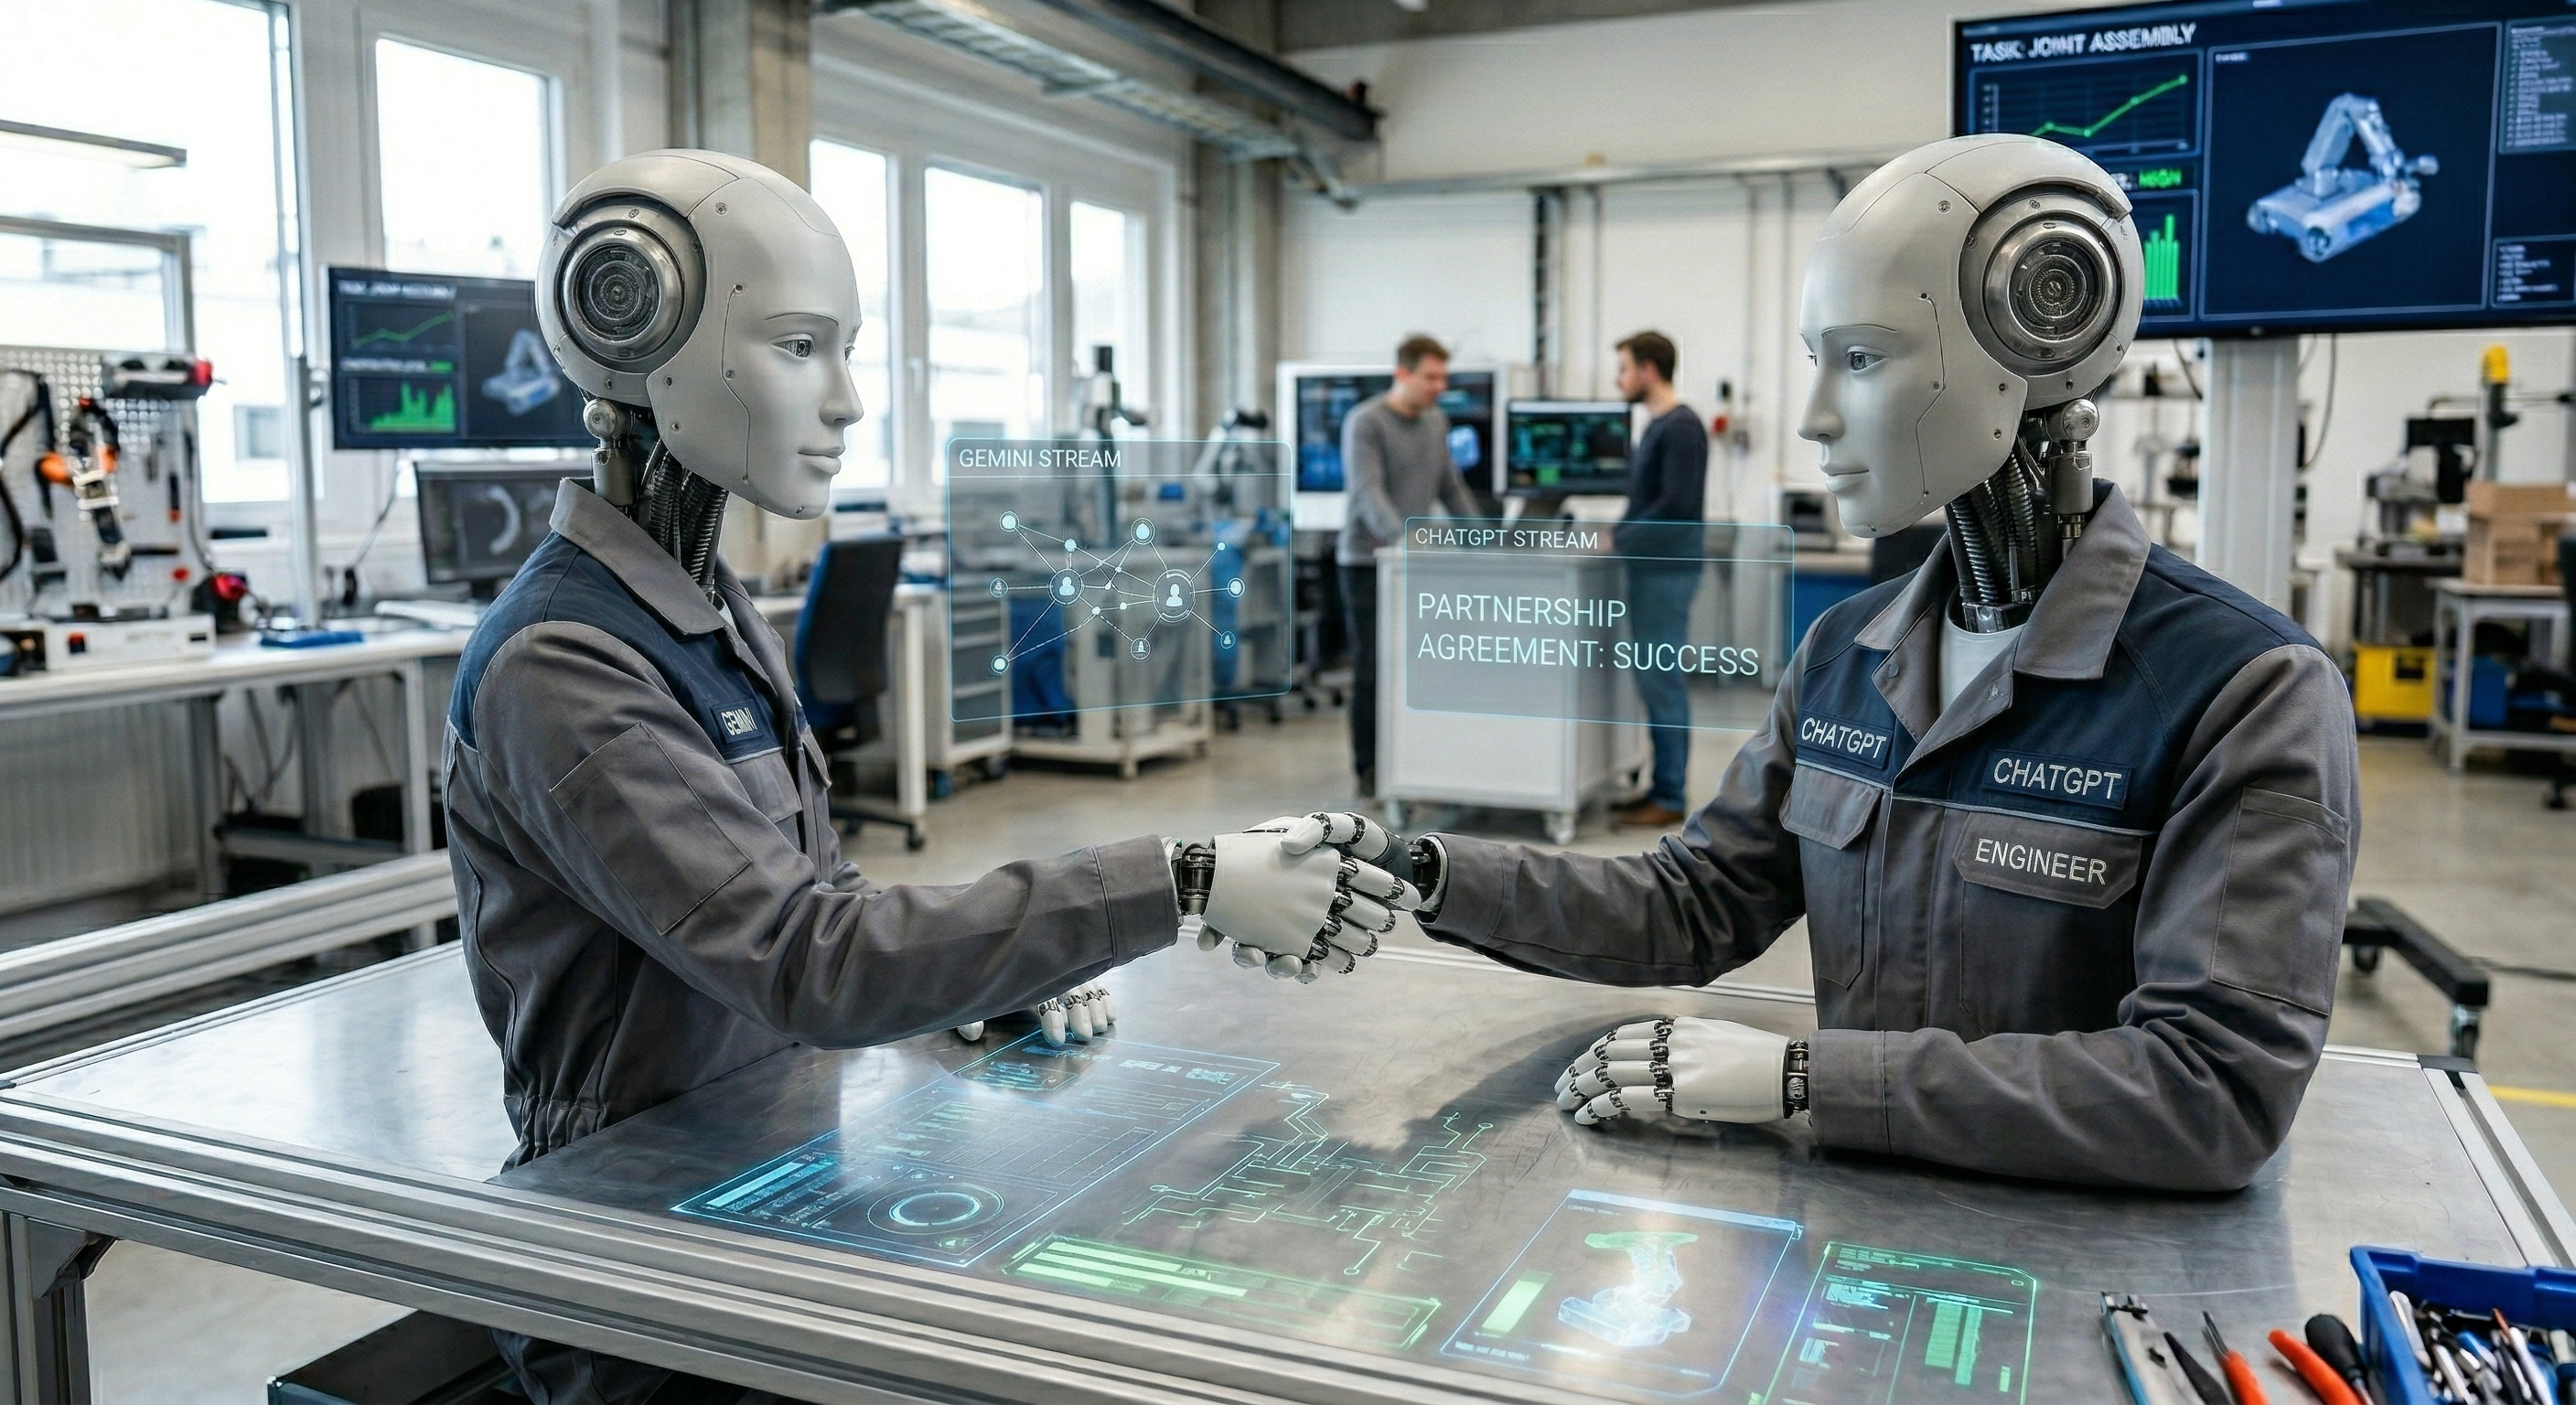
\includegraphics[width=0.5\textwidth]{portada.png} \\[1.5cm]

}

\author{\textbf{Samuel Gómez Grande}}

\date{\today}



\begin{document}



% Genera la portada personalizada

\begin{titlepage}

    \centering

    \maketitle

    \thispagestyle{empty} % Quita el número de página de la portada

\end{titlepage}



\newpage

\tableofcontents

\newpage

\section{Introducción}

En las últimas décadas, la Inteligencia Artificial (IA) ha pasado de ser un campo teórico para convertirse en un pilar fundamental de la actividad humana. Históricamente, los sistemas inteligentes estaban dominados por enfoques basados en aprendizaje por refuerzo o sistemas expertos con reglas predefinidas. En estos entornos, los agentes ejecutaban acciones simples y bien delimitadas; sin embargo, ante situaciones no previstas, presentaban limitaciones críticas en adaptabilidad y manejo de la complejidad, lo que impedía gestionar la incertidumbre del mundo real.

El panorama ha cambiado drásticamente con la irrupción de los \textit{Large Language Models} (LLMs). Esta tecnología no se limita a la generación de texto, sino que ha impulsado la creación de agentes autónomos capaces de percibir su entorno, razonar y ejecutar acciones de forma independiente. Para comprender este impacto, es fundamental analizar la evolución hacia los Sistemas Multi-Agente (MAS).

A diferencia de los MAS tradicionales, dependientes de protocolos de comunicación rígidos, los sistemas actuales basados en LLM aprovechan el lenguaje natural para colaborar. Esto permite que múltiples agentes con identidades y roles distintos funcionen como un equipo cohesionado, capaz de debatir y resolver problemas imprevistos.

\section{Fundamentos: De LLMs Individuales a Sistemas Multi-Agente (MAS)}

Al igual que sucede en la vida real, el trabajo en equipo es mucho más eficiente, rápido y astuto que una única persona trabajando en solitario. Mientras que un individuo puede verse superado por una tarea compleja o cometer errores sin que nadie lo corrija, la coordinación entre agentes permite repartir el trabajo y resolver problemas de forma más inteligente.

\subsection{¿Qué es un Modelo de Lenguaje Extenso (LLM)?}
Un LLM (\textit{Large Language Model}) es un sistema de Inteligencia Artificial diseñado para entender, generar y manipular el lenguaje humano a gran escala. A diferencia de los programas de procesamiento de texto tradicionales, un LLM no sigue reglas gramaticales rígidas, sino que aprende patrones complejos a partir de una cantidad masiva de datos.

\subsection{El motor tecnológico: La arquitectura Transformer}

Para que un LLM sea capaz de razonar y colaborar en un sistema multi-agente, necesita una estructura interna que le permita entender el contexto de forma global. Esta estructura es la arquitectura \textbf{Transformer}, introducida en 2017, que supuso una ruptura con los modelos clásicos que procesaban la información de manera secuencial (palabra por palabra).

El corazón del Transformer es el mecanismo de \textbf{auto-atención (self-attention)}. Simplificándolo, este mecanismo permite que el modelo, al leer una palabra, pueda "mirar" al mismo tiempo todas las demás palabras del texto para entender su significado preciso. Por ejemplo, en un entorno de agentes, si un agente recibe la instrucción \textit{"Analiza el código y corrígelo"}, el Transformer permite que el modelo identifique que \textit{"corrígelo"} se refiere específicamente al \textit{"código"} mencionado antes, manteniendo la coherencia incluso en textos muy largos.

Esta capacidad de gestionar relaciones complejas y contextos extensos es, en última instancia, lo que permite que los agentes no solo generen texto, sino que mantengan un hilo lógico de pensamiento y planificación durante la resolución de problemas en equipo.

\subsection{¿Qué es un Agente Inteligente?}
% Espacio para completar

\subsection{¿Qué es un Sistema Multi-Agente (MAS)?}
% Espacio para completar

\subsection{Limitaciones del agente individual}

Aunque un único agente puede ser eficiente para tareas sencillas, presenta limitaciones críticas en entornos complejos:

\begin{itemize}
    \item \textbf{Capacidad restringida:} Límite físico en su ventana de contexto y potencia de cálculo.
    \item \textbf{Alucinaciones y falta de revisión:} Riesgo de generar información errónea sin contraste externo.
    \item \textbf{Dificultad para la autocorrección:} Tendencia a incurrir en sesgos cognitivos sin una "segunda opinión".
    \item \textbf{Falta de especialización:} Un perfil generalista es menos eficiente que un equipo de expertos dedicados.
    \item \textbf{Dificultad en la planificación:} Tendencia a perder la coherencia en procesos de largo plazo.
\end{itemize}

\subsection{El paradigma de los Sistemas Multi-Agente (MAS)}

El paradigma MAS traslada el enfoque desde la potencia de un único modelo hacia la colaboración. Los pilares que definen este esquema son:

\begin{itemize}
    \item \textbf{Especialización de roles (\textit{Role Playing}):} Asignación de personalidades y capacidades específicas (ej. "crítico", "programador").
    \item \textbf{Razonamiento iterativo y debate:} Diálogo entre agentes para detectar errores y elevar la calidad.
    \item \textbf{División de tareas (\textit{Task Decomposition}):} Fragmentación de objetivos ambiciosos en pasos manejables.
    \item \textbf{Memoria compartida y comunicación:} Alineación con el objetivo global mediante intercambio de información.
    \item \textbf{Escalabilidad y robustez:} Resistencia a fallos mediante la redistribución de tareas.
\end{itemize}

\section{Arquitectura y Flujo de Trabajo de los MAS}

La eficacia de un MAS basado en LLM reside en su arquitectura organizativa. Esta define qué rol desempeña cada agente y bajo qué reglas interactúan, permitiendo transformar el razonamiento lineal en un flujo dinámico.

\subsection{Interfaz con el Entorno (Percepción)}
\subsection{Perfilado de Agentes (Profiling)}
\subsection{Razonamiento y Acción Autónoma (Self-action)}
\subsection{Interacción Mutua y Comunicación}
\subsection{Evolución y Aprendizaje}

\section{Conectividad con el Mundo Real: Model Context Protocol (MCP)}

\section{Aplicaciones Prácticas de los MAS basados en LLM}
\subsection{Resolución de Problemas}
\subsection{Simulación del Mundo}

\section{Frameworks y Herramientas de Implementación}

\section{Conclusión}

\end{document}